\documentclass[../598comp.tex]{subfiles}


\graphicspath{ {./lectures/images/}{./images/} }

\date{05-14}

\begin{document}

\section{05-14}

\subsection{Learning Automata}

Dana Angluin (1987)

Model.  She assumed the existence of a teacher: minimally adequat teacher.

It's always regular languages. Trying to learn a DFA. You can ask ``is $w$ in
L?''.

After collecting some information you propose an answer. A teacher says ``Yes''
or ``No'' and here is a counter example: a word in $L$ that your proposed machine
rejects or a word not in $L$ which your machine incorrectlys accepts. Teacher's
choice not yours.

\begin{theorem}
  With polynomially man queries you are guaranteed to learn the correct unique
  \ul{minimal} DFA for $L$ (even if teacher has a different more complex version).  
\end{theorem}

Basic data structure: Observation table. $S, E \subseteq \Sigma^*$, both finite.
Helpful to think of $S$ as states and $E$ as experiments.
\\\\
Assume you have a table with certain properties satisfied. We can propose a DFA

An observation table is said to be \ul{closed} when
\begin{gather*}
  \forall t \in S \cdot \Sigma, \ \exists s \in S \ s.t. \ row(t) = row(s)
\end{gather*}
An observation table is \ul{consistent} when
\begin{gather*}
  \forall s_1, s_2 \in S, row(s_1) = row(s_2) \Rightarrow \forall a \in \Sigma \
  row(s, a) = row(s_2, a)
\end{gather*}
An observation table desribes a DFA iff it is closed and consistent.
\\\\
Algorithm:
\begin{enumerate}
\item 
  When it's not closed, you ask for more queries.
\item
  When it's not consistent, you expand the number of experiments.
\item
  When it's closed and consistent, you present your DFA. If it's wrong, you use
  the counter example to expand the table and start over.
\end{enumerate}

\begin{example}
  This is an extended example going through the process of finding the DFA. I
  won't write it down. These
  \href{https://cs.mcgill.ca/~prakash/Courses/598/Notes/ariella_notes_learning_automata.pdf}{notes}
  do a great job 
\end{example}
A similar algorithm works for weighted automata.
\\\\
This is kinda automata theory meets machine learning. Another application is in
trying to understand what an RNN does. The question of interpreting what an RNN
does once it has been trained. It's important to have explainable AI.
\\\\
Idea: Use an RNN as the teacher and extract a DFA as the explanation of what the
RNN is doing. Gail Weiss. Alika Utepoua and Prakash are exploring this.

\subsection{Fixed Point Operators and LTL}

$\square \varphi = O \varphi \wedge OO \varphi \cdots$

This leads to infinitely many conjunctions. We should be able to prove this with
induction.
\\\\
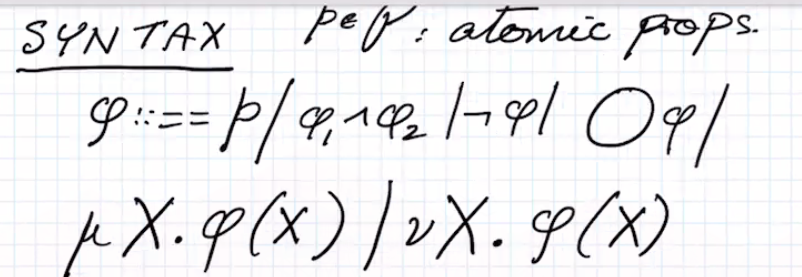
\includegraphics[width=\textwidth]{syntax_fixed.png}

$X$ is a \ul{new} syntacting entity. It is a variable that can range over
formulas. $\mu X$ and $\nu X$ are variable \ul{binders}.  They are called fixed
point operators.
\begin{recall}
  Every monotone function from a complete lattice to itself has a least fixed
  point and a greatest fixed point. $\mu$ stands for least fixed point. $\nu$
  stands for greatest fixed point.
\end{recall}
We are \ul{not} allowed to put a fixed point operator binding an $X$ unless $X$
appears in the scope of an even number of negations.
\\\\
$\mu X . \varphi \wedge \neg X$ and $\mu X. X \Rightarrow \varphi$
are not allowed because they involve negated $X$. Remember that $x \Rightarrow y
$ is the same as $\neg x \vee y$.
\\\\
We defined the semantics in terms of sequences $\sigma \models \varphi$.
\begin{gather*}
  \llbracket \varphi \rrbracket = \{ \sigma \ | \ \sigma \models \varphi \}
\end{gather*}
gives a definable set. Given a formula with a \ul{free} variable, we interpret
it not as a set but as a function from sets to sets.
\begin{gather*}
  \llbracket \varphi(X) \rrbracket = S \mapsto \llbracket \varphi [S / X] \rrbracket
\end{gather*}
$\varphi[S / X]$ notation for substitute the set $S$ regarded as a formula for
$X$ in $\varphi$.
\\\\
e.g. $\varphi(X) = \psi \wedge OX$.
\\\\
$\llbracket \varphi(X) \rrbracket(S) = \{\sigma \ | \ \sigma \models \psi \wedge
\sigma[1..] \in S\}$
\\\\
\begin{fact}
  With the restriction these functions are always monotone and
  $P(\Sigma^\omega)$ is a complete lattice.
\end{fact}
Now we define
\begin{gather*}
  \llbracket \mu X.\varphi(X) \rrbracket = lfp\llbracket \varphi(X) \rrbracket
  \\
  \llbracket \nu X. \varphi(X) \rrbracket = gfp \llbracket \varphi(X) \rrbracket
\end{gather*}
It's a nightmare to interpret nested fixed points in human terms (although it is still well defined).
\\\\
$\square \varphi = \nu X. \varphi \wedge OX$
\\
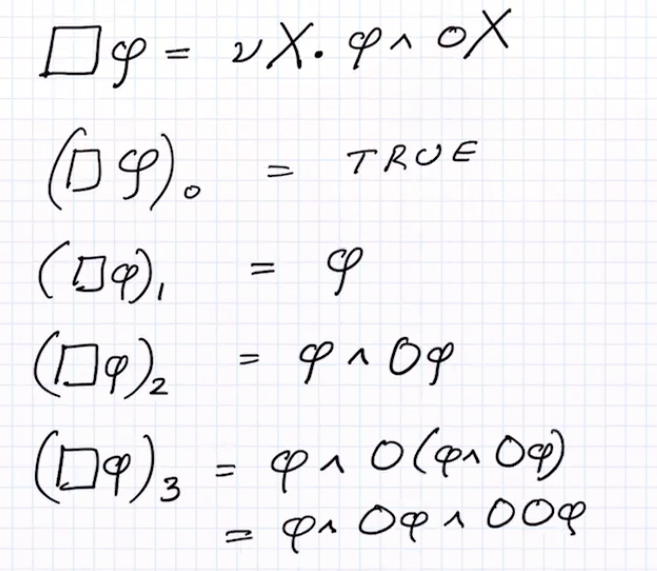
\includegraphics[width=\textwidth]{boxphi_breakdown.png}





\end{document}